%
% $RCSfile: counted_pointer.tex,v $
%
% Copyright (C) 2002-2008. Christian Heller.
%
% Permission is granted to copy, distribute and/or modify this document
% under the terms of the GNU Free Documentation License, Version 1.1 or
% any later version published by the Free Software Foundation; with no
% Invariant Sections, with no Front-Cover Texts and with no Back-Cover
% Texts. A copy of the license is included in the section entitled
% "GNU Free Documentation License".
%
% http://www.cybop.net
% - Cybernetics Oriented Programming -
%
% http://www.resmedicinae.org
% - Information in Medicine -
%
% Version: $Revision: 1.1 $ $Date: 2008-08-19 20:41:06 $ $Author: christian $
% Authors: Christian Heller <christian.heller@tuxtax.de>
%

\subsubsection{Counted Pointer}
\label{counted_pointer_heading}
\index{Counted Pointer Pattern}
\index{Memory Management in C++}
\index{Garbage Collector}

The \emph{Counted Pointer} pattern \cite{buschmann} supports memory management
in the \emph{C++} programming language, by counting references to dynamically
created objects (figure \ref{pointer_figure}). That way, it can avoid the
destruction of an object through one client, while still being referenced by
other clients. Also, it helps avoiding memory leaks by cleaning up forgotten
objects in the style of a \emph{Garbage Collector}.

\begin{figure}[ht]
    \begin{center}
        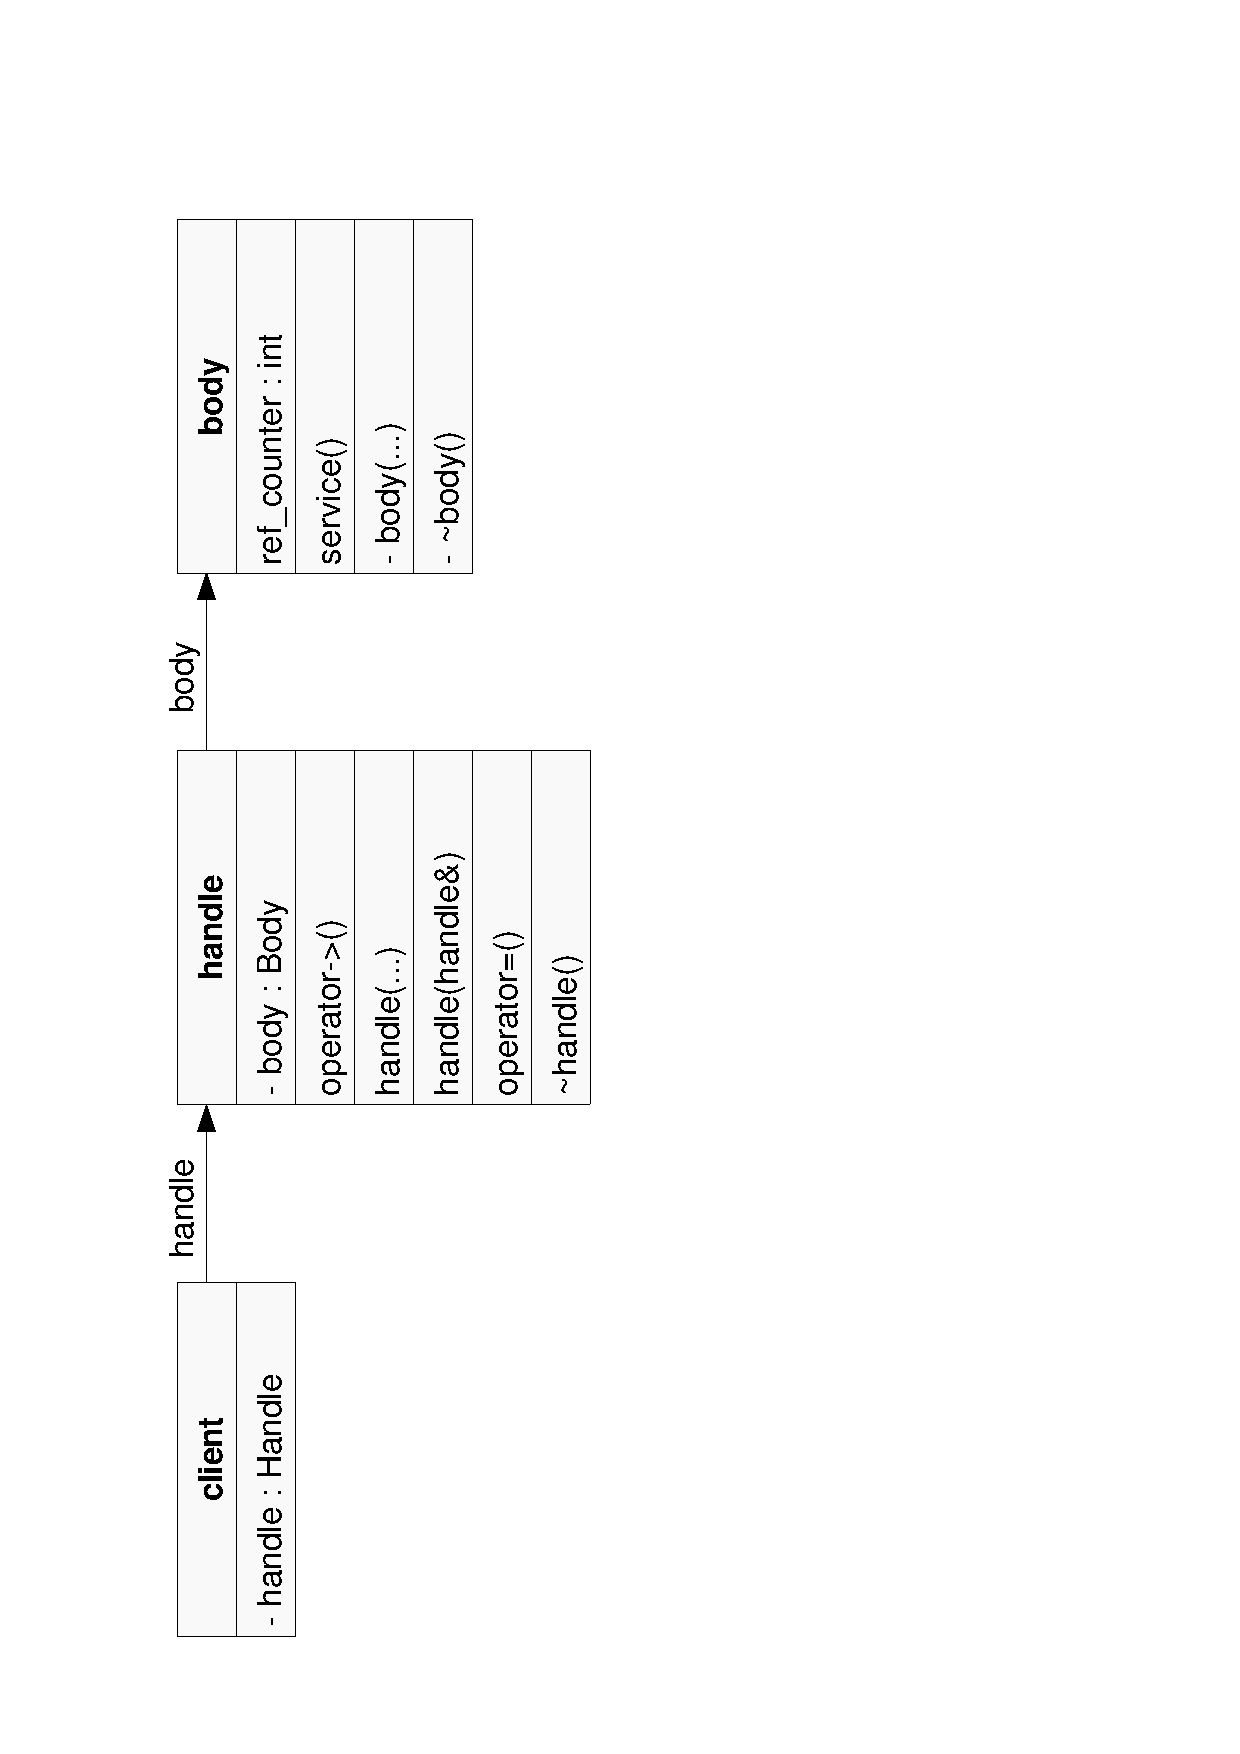
\includegraphics[scale=0.3,angle=-90]{graphic/pointer.pdf}
        \caption{Counted Pointer Pattern}
        \label{pointer_figure}
    \end{center}
\end{figure}

Since all of its knowledge is kept in just one huge tree structure, the
interpreter introduced in chapter \ref{cybernetics_oriented_interpreter_heading}
has memory management and reference counting capabilities built in by default.
